\documentclass[11pt]{report}
\usepackage{amsthm}
\usepackage{amssymb, amsmath}
\usepackage{array}
%\usepackage[romanian]{babel}
\usepackage{bm}
\usepackage{enumerate}
\usepackage{geometry}
\usepackage{graphicx}
\usepackage{index}
%\usepackage{tikz}
\usepackage{ucs}
\usepackage[utf8]{inputenc}

\theoremstyle{plain}
\newtheorem{theorem}{Theorem}

\theoremstyle{definition}
\newtheorem{definition}{Definition}

\theoremstyle{definition}
\newtheorem{lemma}{Lemma}

\theoremstyle{proposition}
\newtheorem{proposition}{Proposition}

 \geometry{
 a4paper,
 total={160mm,257mm},
 left=30mm,
 right=20mm,
 top=20mm,
 bottom=20mm,
 }
 
\renewcommand{\baselinestretch}{1}
 
\graphicspath{ {Imagini/} }

\begin{document}

\begin{titlepage}

\begin{center}
\begin{large}
Universitatea ``Alexandru Ioan Cuza" din Iaşi\\
Facultatea de Informatică\\
\end{large}
\end{center}

\vspace{50mm}

\begin{center}

\includegraphics{fii.png}
\end{center}
 
\vspace{15mm}

\begin{center}
\begin{Large}
LUCRARE DE DISERTAŢIE
\end{Large}
\\
\
\\
\
\

\begin{Huge}
\textbf{Awesome Name}
\end{Huge}

\

propusă de

\end{center}

\vspace{30mm}

\textbf{Student:} Oriana-Maria Oniciuc

\textbf{Coordonator ştiinţific:} Conf. Dr. Liviu Ciortuz
\\
\
\\
\


\vfill

\begin{center}
\textbf{Sesiunea:} iulie

2018
\end{center}

\end{titlepage}
\newpage

\begin{titlepage}

\begin{center}
Universitatea ``Alexandru Ioan Cuza" din Iaşi\\
Facultatea de Informatică\\
\end{center}

\vspace{85mm}
 
\begin{center}
\begin{Huge}
\textbf{Awesome Name}
\end{Huge}
\end{center}
 
\vspace{60mm}

\textbf{Student:} Oriana-Maria Oniciuc

\textbf{Coordonator ştiinţific:} Conf. Dr. Liviu Ciortuz

\vfill

\begin{center}
\textbf{Sesiunea:} iulie

2018
\end{center}

\end{titlepage}
\newpage

\

\pagenumbering{arabic}

\vspace{10mm}
\begin{large}
\begin{center}
DECLARAŢIE PRIVIND ORIGINALITATE ŞI RESPECTAREA DREPTURILOR DE AUTOR
\end{center}
\end{large}

\vspace{20mm}

Prin prezenta declar că Lucrarea de disertaţie cu titlul ``Awesome Name” este scrisă de mine şi nu a mai fost prezentată niciodată la o altă facultate sau instituţie de învăţământ superior din ţară sau străinătate. De asemenea, declar că toate sursele utilizate, inclusiv cele preluate de pe Internet, sunt indicate în lucrare, cu respectarea regulilor de evitare a plagiatului:

\begin{itemize}
\item toate fragmentele de text reproduse exact, chiar şi în traducere proprie din altă limbă, sunt scrise între ghilimele şi deţin referinţa precisă a sursei;
\item reformularea în cuvinte proprii a textelor scrise de către alţi autori deţine referinţa precisă;
\item codul sursă, imaginile etc. preluate din proiecte open-source sau alte surse sunt utilizate cu respectarea drepturilor de autor şi deţin referinţe precise; 
\item rezumarea ideilor altor autori precizează referinţa precisă la textul original.

\end{itemize}

\vspace{10mm}

Iaşi,
\

XX iunie 2018
\

\begin{flushright}
Absolvent,
\\

Oniciuc Oriana-Maria
\\
\
\

\line(1,0){150}
\

(semnătura în original)
\end{flushright}

\newpage

\

\vspace{20mm}
\begin{large}
\begin{center}
DECLARAŢIE DE CONSIMŢĂMÂNT
\end{center}
\end{large}

\vspace{30mm}

Prin prezenta declar că sunt de acord ca Lucrarea de disertaţie cu titlul ``Awesome Name”, codul sursă al programelor şi celelalte conţinuturi (grafice, multimedia, date de test etc.) care însoţesc această lucrare să fie utilizate în cadrul Facultăţii de Informatică.
\\

De asemenea, sunt de acord ca Facultatea de Informatică de la Universitatea ``Alexandru Ioan Cuza” din Iaşi să utilizeze, modifice, reproducă şi să distribuie în scopuri necomerciale programele-calculator, format executabil şi sursă, realizate de mine în cadrul prezentei lucrări de disertaţie.

\vspace{20mm}

Iaşi,
\

XX iunie 2018
\\
\

\begin{flushright}
Absolvent,
\\

Oniciuc Oriana-Maria
\\
\
\

\line(1,0){150}
\

(semnătura în original)
\end{flushright}

\newpage

\vspace{10mm}
\begin{abstract}
\

This paper aims is to produce a method that classifies phonocardiograms corresponding to different heart symptoms that are extremely subtle and challenging to separate. The problem is of particular interest to machine learning researchers as it involves classification of audio sample data, where distinguishing between classes of interest is non-trivial. Data is gathered in real-world situations and frequently contains background noise of every conceivable type. Despite its medical significance, to date this is a relatively unexplored application for machine learning.
\\

Some attempts to segment phonocardiograms (PCG) into heartbeats can be
found in the literature. The characteristics of the PCG signal and other features
such as heart sounds S1 and S2 location can be measured more accurately by digital signal processing techniques. Basic frequency content of PCG signal can be
easily provided using Fast Fourier Transform technique. However, time duration
and transient variation cannot be resolved just through FFT, and in this case the
Continuous Wavelet Transform is a more suitable technique to analyze such a signal. The coefficients of the CWT give a graphic representation that is very helpful
in extracting quantitative analysis simultaneously in time and frequency.
\\

For the classification task some of the representative work that was done, has been presented in Classifying Heart Sounds Workshop. The teams used the J48 and MLP algorithms (using Weka) to train and classify the computed features, or exploit domain knowledge and compares the features of heartbeat before and after dropping out extra peaks and the smallest interval, used partial least squares regression, neural networks and convolution neural networks. The classification task in this project aims to give an alternative architecture for the convolution neural network proposed in Classification of Heart Sound Recordings using Convolution Neural Network.
\end{abstract}

\newpage
%\pagenumbering{gobble}
%\

%\vspace{60mm}
%\
%
%\textbf{Mulţumiri}
%\\
%
%\
%
%Îmi doresc să mulţumesc celor care m-au susţinut în conceperea acestei lucrări. Sunt pe deplin recunoscătoare coordonatorului ştiinţific, conf. dr. Cristian Gaţu. Am învăţat foarte multe de la dumnealui şi m-a ghidat de fiecare dată spre rezultate foarte bune. Vreau să mulţumesc şi întregului corp profesoral care m-a îndrumat în aceşti ani nu doar ca excelenţi dascăli, ci mai ales ca modele pentru o carieră viitoare. De asemenea sunt recunoscătoare dragei mele familii şi tuturor colegilor extraordinari care mi-au fost alături în tot acest timp.
%
%\clearpage
%
%\newpage
\pagenumbering{arabic}
\setcounter{page}{5}
\addcontentsline{toc}{chapter}{Contents}

\tableofcontents

\newpage

\addcontentsline{toc}{chapter}{I. Introduction}
\chapter*{I. Introduction}

\

According to the World Health Organization, cardiovascular diseases are the
number one cause of death globally. These diseases have remained the leading
causes of death in the last 15 years. Any work done in detecting signs of heart
disease could therefore have a significant impact on world health.
\\

Classifying Heart Sounds PASCAL provides us with a dataset that is gathered
in real-world situations and frequently contains background noise of every con-
ceivable type, being recorded both in a Hospital environment by a doctor (using a
digital stethoscope) and at home by the patient (using a mobile device). Success in
classifying this form of data requires multiples preprocessing of the audio record-
ings. This part of the research presents an overview of approaches to analysis of
heart sound signals. The main purpose of this study is developing an automatic
methodology for identifying systole and diastole in the phonocardiograms and to
classify the heartbeats in three classes.
\\


\addcontentsline{toc}{section}{I.1. Heart sounds}
\section*{II.1. Heart sounds}

\

The cardiac cycle is the performance of the human heart from the beginning of one heartbeat to the beginning of the next. It consists of two periods: one during which the heart muscle relaxes and refills with blood, called diastole, followed by a period of robust contraction and pumping of blood, dubbed systole. After emptying, the heart immediately relaxes and expands to receive another influx of blood returning from the lungs and other systems of the body—before again contracting to pump blood to the lungs and those systems.
\\

Mechanical vibrations reflect the turbulence that occurs
when heart valves close. Traditionally, a stethoscope is used in
cardiac auscultation to listen to these sounds that provide
important acoustic information regarding the condition of the heart.
Phonocardiography, diagnostic technique that creates a graphic record, or phonocardiogram, of the sounds and murmurs produced by the contracting heart, including its valves and associated great vessels. The phonocardiogram is obtained either with a chest microphone or with a miniature sensor in the tip of a small tubular instrument that is introduced via the blood vessels into one of the heart chambers. The phonocardiogram usually supplements the information obtained by listening to body sounds with a stethoscope (auscultation) and is of special diagnostic value when performed simultaneously with measurement of the electrical properties of the heart (electrocardiography) and pulse rate.
\\


The time-frequency analysis of the PCG signals permits detecting and characterising abnormal murmurs or extra in the diagnosis of heart disease. In this study, we analyse normal, murmur and extra heart sounds recordings, separating them from artifacts. Most often, the symptoms of cardiovascular diseases become worse over time and detecting them in early stages is crucial.
\\

The corelation among the phonocardiogram and the biological phenomenom is presented in the following diagram:

\begin{figure}[h]
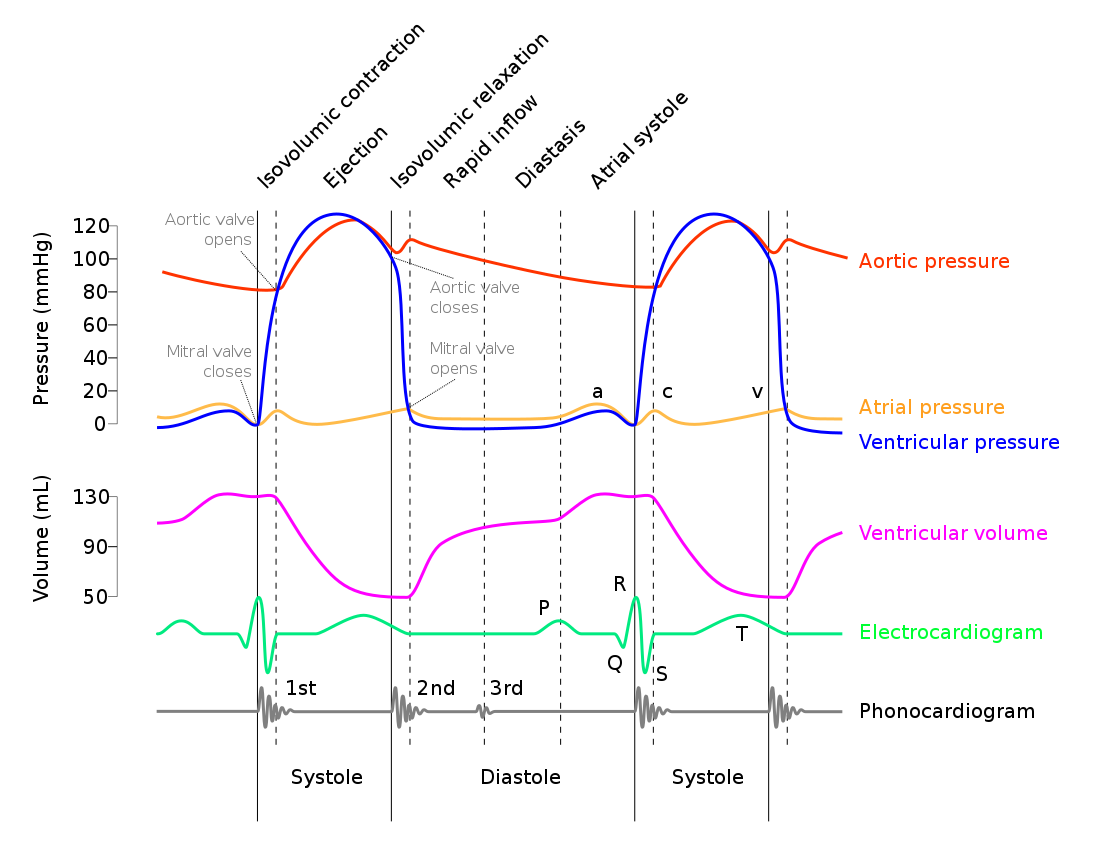
\includegraphics[width=15cm]{Wiggers_Diagram_2.png}
\centering
\caption{The Wiggers diagram clearly illustrates the coordinated variation of these values as the heart beats, assisting one in understanding the entire cardiac cycle.}
\end{figure}

\textbf{Heart murmur}
\\

Heart murmurs are heart sounds produced when blood flows across one of the heart valves that are loud enough to be heard with a stethoscope. Heart murmurs are most frequently categorized by timing, into systolic heart murmurs and diastolic heart murmurs, differing in the part of the heartbeat on which they can be heard. However, continuous murmurs cannot be directly placed into either category.
\\

Systolic murmurs are due to blood flow through the semilunar valves. They occur at the start of blood ejection — which starts after S1 — and ends with the cessation of the blood flow — which is before S2. Diastolic murmurs start after S2 and end before S1. Many involve stenosis of the atrioventricular valves or regurgitation of the semilunar valves.
\\

\textbf{Heart arrhythmia}
\\

Heart arrhythmia (also known irregular heartbeat) is a group of conditions in which the heartbeat is irregular, too fast, or too slow. There are four main types of arrhythmia: extra beats, supraventricular tachycardias, ventricular arrhythmias, and bradyarrhythmias. Extra beats, the disease included in our dataset, include premature atrial contractions, premature ventricular contractions, and premature junctional contractions.


\addcontentsline{toc}{section}{I.2. Previous work}
\section*{II.2. Previous work}
\

Many studies have been done on PCG signal sofar. The research on this topic ncreased nowadays due to improvement in signal processing techniques and new methods in big data analysis. A summary of the most important results obtained with the Classifying Heart Sounds PASCAL Challenge dataset can be found here[].
\\

The Classifying Heart Sounds Workshop 2012 is the first international workshop to focus on the use of statistical machine learning techniques to segment and classify real-world heart audio. The clallange for this workshop was to create a first level of screening of cardiac pathologies both in a Hospital environment by a doctor (using a digital stethoscope) and at home by the patient (using a mobile device). 
\\

The problem is of particular interest to machine learning researchers as it involves classification of audio sample data, where distinguishing between classes of interest is non-trivial. Success in classifying this form of data requires extremely robust classifiers. 
\\

\begin{figure}[h]
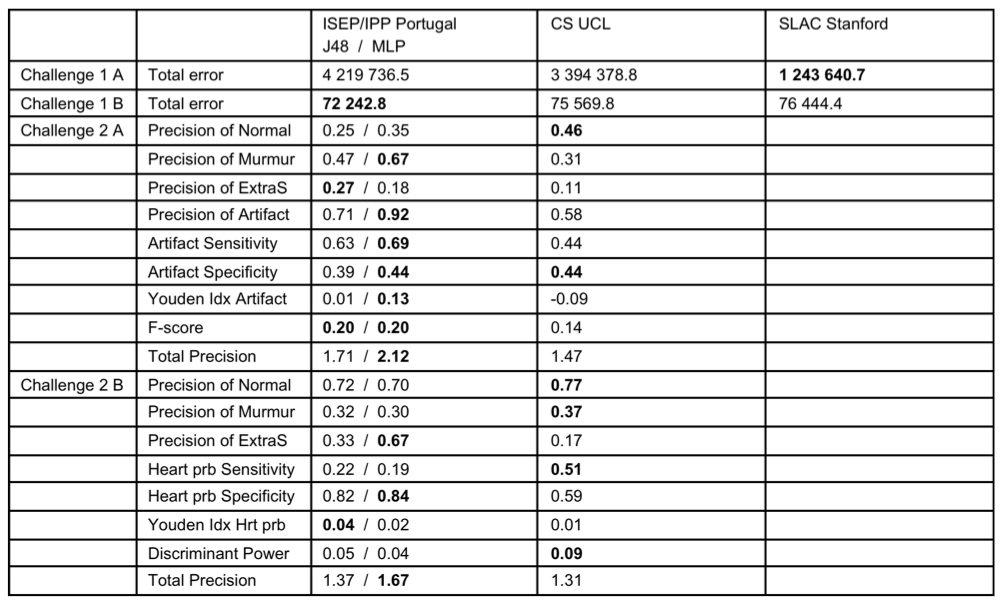
\includegraphics[width=14.5cm]{challengeresults.png}
\centering
\caption{A summary of the results of the three finalists from their approaches}
\end{figure}

The first team uses, after the segmentation, the J48 and MLP algorithms (using Weka) to train and
classify the computed features. The UCL team exploits domain knowledge and
compares the features of heartbeat before and after dropping out extra peaks and
the smallest interval. By doing so they try to minimize the negative effect of noise.
In the literature there are other proposed ways to tackle this challenge: partial
least squares regression, neural networks and convolution neural networks.
\\

Other models for classifing the heart sounds can be found [kaggle], where the best general accuracy obtained was $93,18 \%$ for all the classes. The model proposed is a neural network.


\newpage



\addcontentsline{toc}{chapter}{II. Methodology and research methods}
\chapter*{II. Methodology and research methods}

\addcontentsline{toc}{section}{II.1. CRISP-DM Methodology}
\section*{II.1. CRISP-DM Methodology}

\

Cross-industry standard process for data mining, commonly known by its acronym CRISP-DM, is a data mining process model that describes commonly used approaches that data mining experts use to tackle problems. CRISP-DM breaks the process of data mining into six major phases.
\\

The sequence of the phases is not strict and moving back and forth between different phases as it is always required. The arrows in the process diagram indicate the most important and frequent dependencies between phases. The outer circle in the diagram symbolizes the cyclic nature of data mining itself. A data mining process continues after a solution has been deployed. The lessons learned during the process can trigger new, often more focused business questions, and subsequent data mining processes will benefit from the experiences of previous ones.
\\

\textbf{Business understanding}

\

This initial phase focuses on understanding the project objectives and requirements from a business perspective, and then converting this knowledge into a data mining problem definition, and a preliminary plan designed to achieve the objectives. A decision model, especially one built using the Decision Model and Notation standard can be used.
\\

\textbf{Data understanding}

\

The data understanding phase starts with an initial data collection and proceeds with activities in order to get familiar with the data, to identify data quality problems, to discover first insights into the data, or to detect interesting subsets to form hypotheses for hidden information.
\\

\textbf{Data preparation}

\

The data preparation phase covers all activities to construct the final dataset (data that will be fed into the modeling tool(s)) from the initial raw data. Data preparation tasks are likely to be performed multiple times, and not in any prescribed order. Tasks include table, record, and attribute selection as well as transformation and cleaning of data for modeling tools.
\\

\textbf{Modeling}

\

In this phase, various modeling techniques are selected and applied, and their parameters are calibrated to optimal values. Typically, there are several techniques for the same data mining problem type. Some techniques have specific requirements on the form of data. Therefore, stepping back to the data preparation phase is often needed.
\\

\textbf{Evaluation}

\

At this stage in the project you have built a model (or models) that appears to have high quality, from a data analysis perspective. Before proceeding to final deployment of the model, it is important to more thoroughly evaluate the model, and review the steps executed to construct the model, to be certain it properly achieves the business objectives. A key objective is to determine if there is some important business issue that has not been sufficiently considered. At the end of this phase, a decision on the use of the data mining results should be reached.
\\

\textbf{Deployment}

\

Creation of the model is generally not the end of the project. Even if the purpose of the model is to increase knowledge of the data, the knowledge gained will need to be organized and presented in a way that is useful to the customer. Depending on the requirements, the deployment phase can be as simple as generating a report or as complex as implementing a repeatable data scoring (e.g. segment allocation) or data mining process. In many cases it will be the customer, not the data analyst, who will carry out the deployment steps. Even if the analyst deploys the model it is important for the customer to understand up front the actions which will need to be carried out in order to actually make use of the created models.
\\



\addcontentsline{toc}{section}{II.2. Data preparation}
\section*{II.2. Data preparation}

\



\addcontentsline{toc}{section}{II.3. Modeling}
\section*{II.3. Modeling}

\

\addcontentsline{toc}{section}{II.4. Technologies}
\section*{II.4. Technologies}

\

\newpage

\addcontentsline{toc}{chapter}{III. Results}
\chapter*{III. Results}


Criptografia a apărut pe vremea egiptenilor, cu peste 4000 de ani în urmă. În principal, până la începutul secolului al XX-lea, criptografia s-a ocupat mai ales de şabloane lingvistice. De atunci, accentul s-a mutat pe folosirea extensivă a matematicii, inclusiv a aspectelor de teoria informaţiei, complexitatea algoritmilor, statistică, combinatorică, algebră abstractă şi teoria numerelor. Din punct de vedere lexicografic, cuvântul \textit{criptografie} este format din rădăcinile \textit{cryptos} şi \textit{grafie}.

\begin{center}
Criptografie = \textit{cryptos}(ascuns) + \textit{grafie}(a scrie)
\end{center}
\

Criptografia este o componentă a domeniului securităţii informaţiei şi poate fi definită astfel:

\begin{definition} \textit{Criprografia} este studiul tehnicilor matematice care se ocupă de următoarele aspecte ale securităţii informaţiei: confidenţialitatea, autentificarea, non-repudierea mesajelor şi integritatea datelor.
\end{definition}
\

Principalele obiective ale unui sistem criptografic sunt:
\begin{itemize}
	\item \textit{Confidenţialitatea}: proprietatea de a păstra secretul informaţiei, astfel încât aceasta să fie utilizată numai de către persoane autorizate.
	\item \textit{Autentificarea}: proprietatea de a identifica o entitate conform anumitor standarde. Aceasta implică:		
	\begin{enumerate}
		\item Autentificarea unei entităţi;
		\item Autentificarea sursei informaţiei.
	\end{enumerate}
	\item \textit{Non-repudierea}: proprietatea care previne negarea unor evenimente anterioare.
	\item \textit{Integritatea datelor}: proprietatea de a evita orice modificare (inserare, ştergere, substituţie) neautorizată a informaţiei.
\
\end{itemize}


\newpage

\addcontentsline{toc}{chapter}{IV. Conclusion}
\chapter*{IV. Conclusion}

\nocite{*}
\addcontentsline{toc}{chapter}{VI. Bibliography}
\bibliographystyle{plain}
\bibliography{bibliografie}

%% F6 F11 F6 F6 Quick Build

\end{document}